\chapter{Chromatic Page:}
The PTC page, also known as the  Chromatic Page is used to play MD tracks chromatically using the MD Trigger interface or an attached MIDI Keyboard.\\
\\For supported track types, the Track’s Pitch is mapped to Notes of a selected scale across the MD Trigger interface.\\
\\Melodies can be recorded in real-time.\\
\\
\fbox{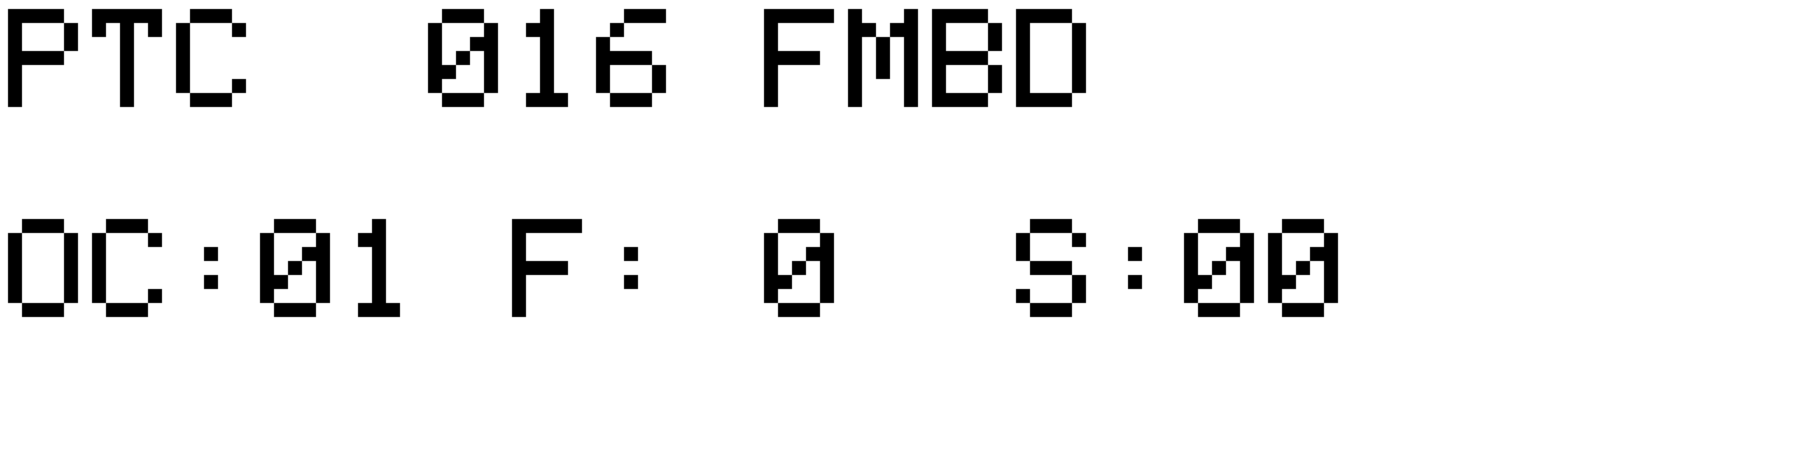
\includegraphics[scale=.40]{ptc_md.png}}\\\\
\textit{To enter the PTC Page: Select desired track on MD by pressing \textbf{[ Function ] + [ Track N ]}. Enter the PTC mode by pressing \textbf{[ Encoder 4 ] }from within the MCL Grid Page.}
\section{Encoder Assignment:}

	\begin{itemize}
		\item \textbf{[ Encoder 1 ]: } Octave (OC)
		\item \textbf{[ Encoder 2 ]: } Fine Tune (F)
		\item \textbf{[ Encoder 3 ]: } Track Length
		\item \textbf{[ Encoder 4 ]: } Scale Type (S)
	\end{itemize}
\section{A4 + ExtMIDI:}
The PTC Page is also used to record/play the Analog4 or ExtMIDI tracks. Scale modes are also supported for these track types.\\
\fbox{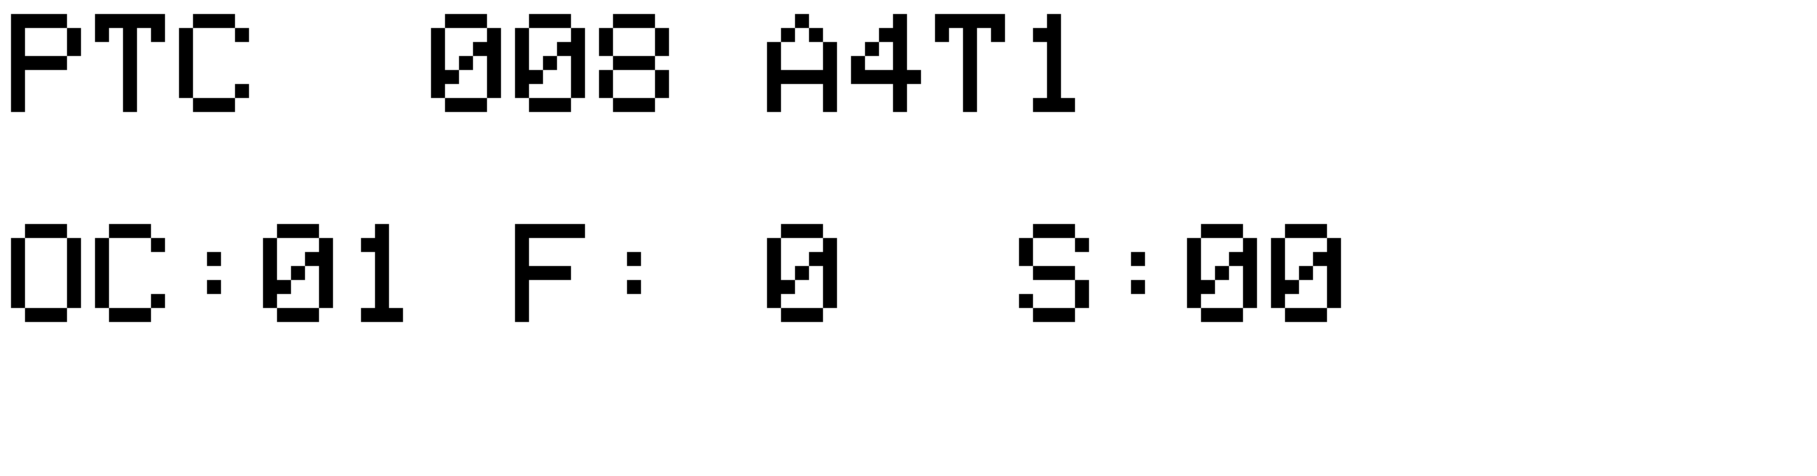
\includegraphics[scale=.40]{ptc_a4.png}}\\
\section{Recording a sequence:}
\textit{Press the \textbf{[ Save ] }button to enable record mode, RPTC.\\}
\\Play notes on either the MD or A4/ExtMidi to record a melody
\section{Clearing Recorded Sequence:}
To clear the current track press the \textbf{[ Write ]}\\
\\To clear all tracks of the current track type press \textbf{[ Shift2 ] + [ Write]}
\section{Changing Track Length:}
Track length is controlled by rotating \textbf{[ Encoder 3 ]}.\\
\\To change the lengths of all tracks of the same track type simultaneously hold down \textbf{[Shift 2] }whilst rotating \textbf{[ Encoder 3 ]}.

\section{A4 or ExtMidi}
Melodies and chords can be played and recorded from the Analog4 or ExtMIDI device in the PTC and RPTC pages.\\
\\
If using the Analog 4, select the desired track using the A4’s track select buttons. The first note played on the mini keyboard will cause the PolyStep edit page to switch to  the corresponding external sequencer track.\\
\\
Switching Between Low and High Resolution Modes on Poly Sequencer Tracks.
Press [ shift2 ] followed by [ shift1 ]

